% !TEX root = main.tex
\newgeometry{
    top=1cm,bottom=1cm,left=1cm,right=1cm
}
\pagestyle{empty}

\vspace*{-0.5cm}
\section{UML Diagrams}
\vspace{2cm}

\begin{figure}[h]
    \centering
    \subfigure[First half]{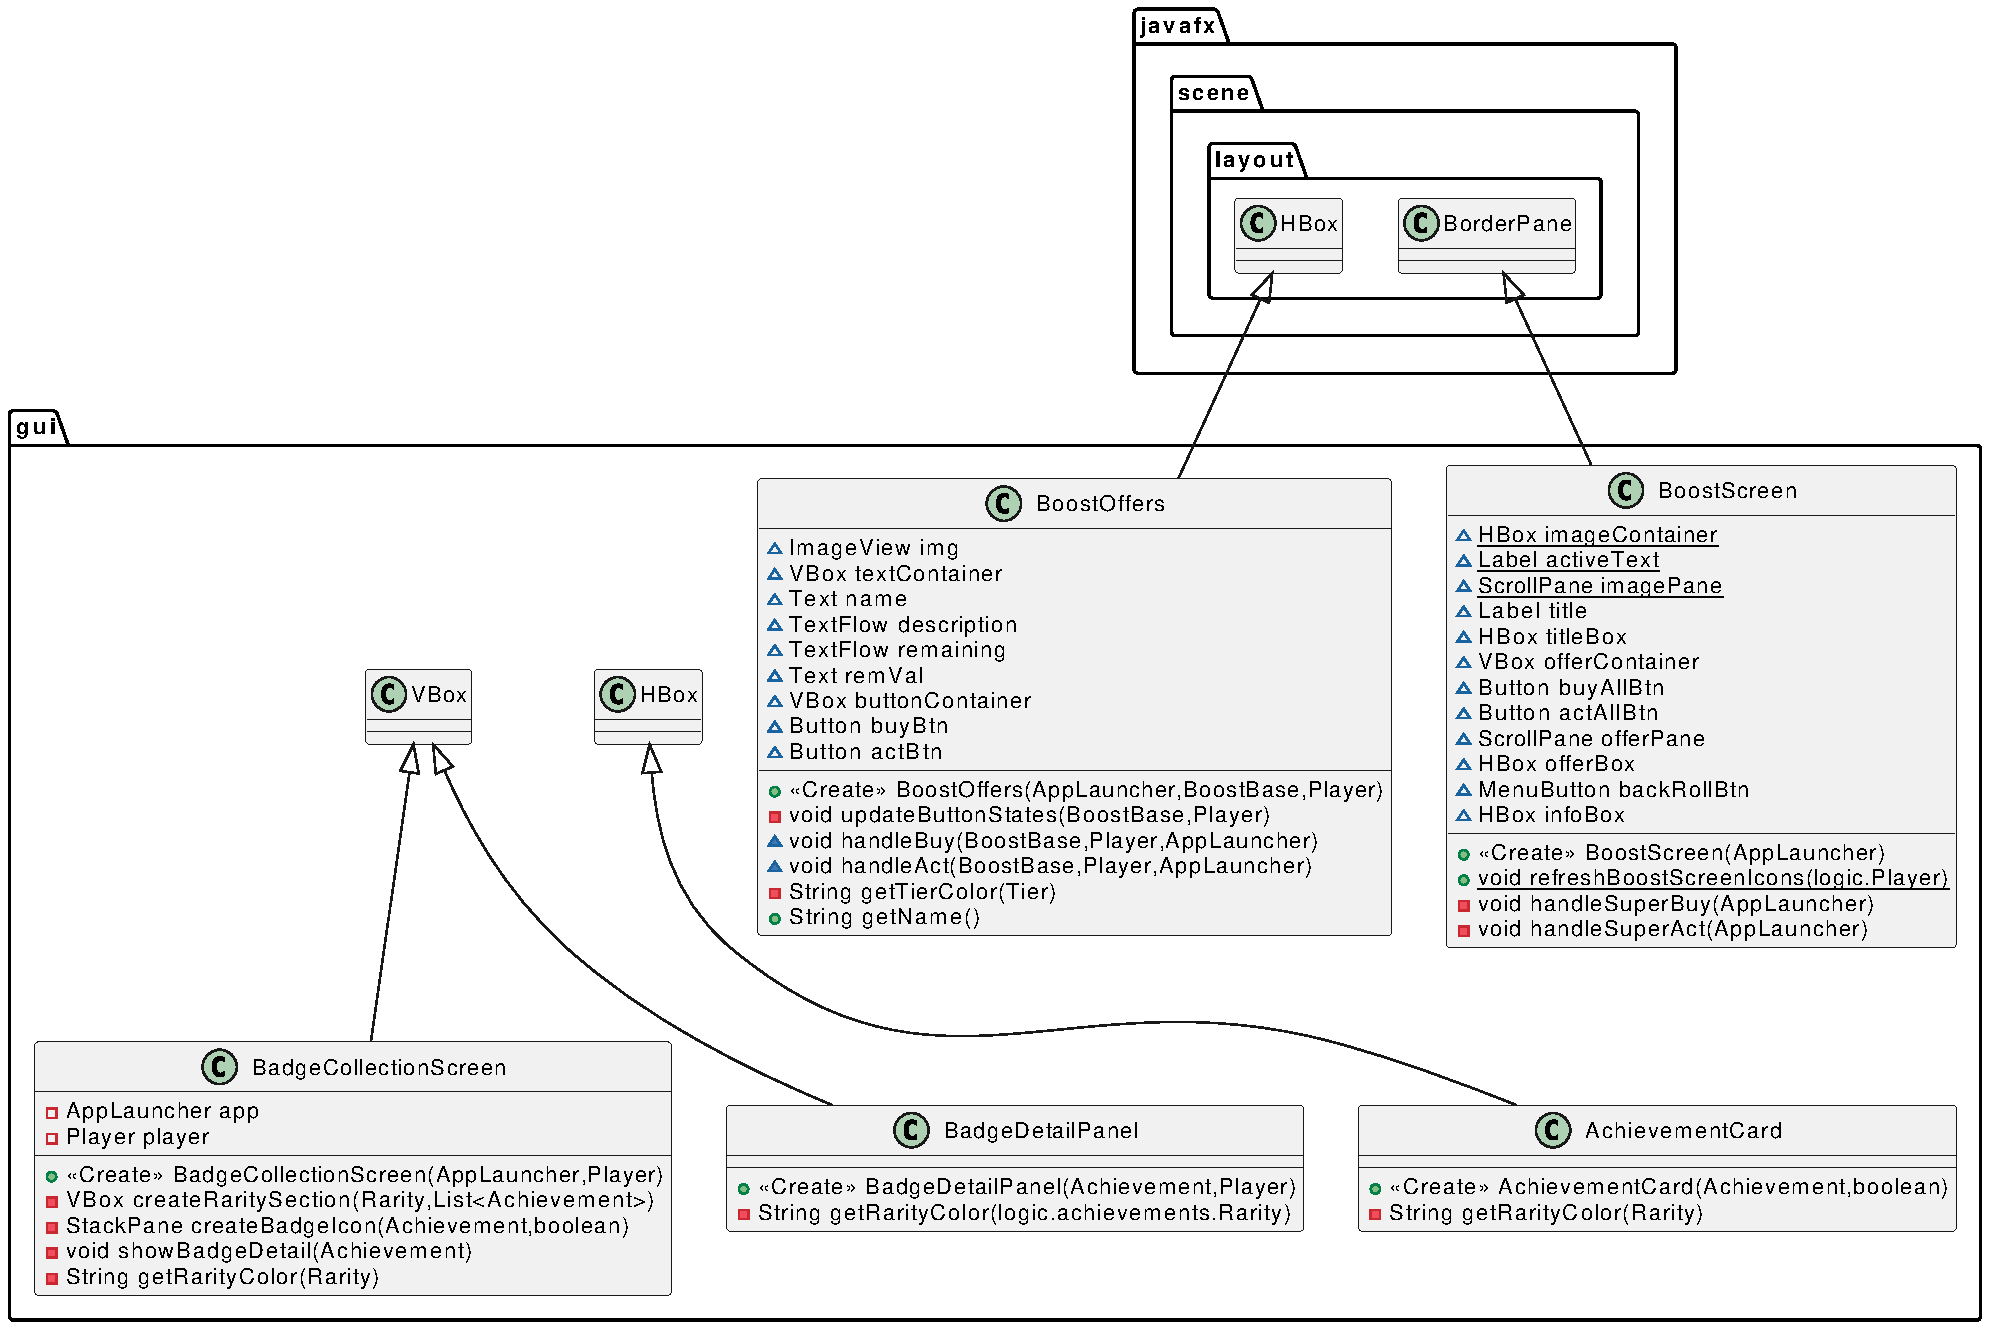
\includegraphics[scale=0.4]{UML/gui1.pdf}}
    \vspace{1.2cm}

    \subfigure[Second half]{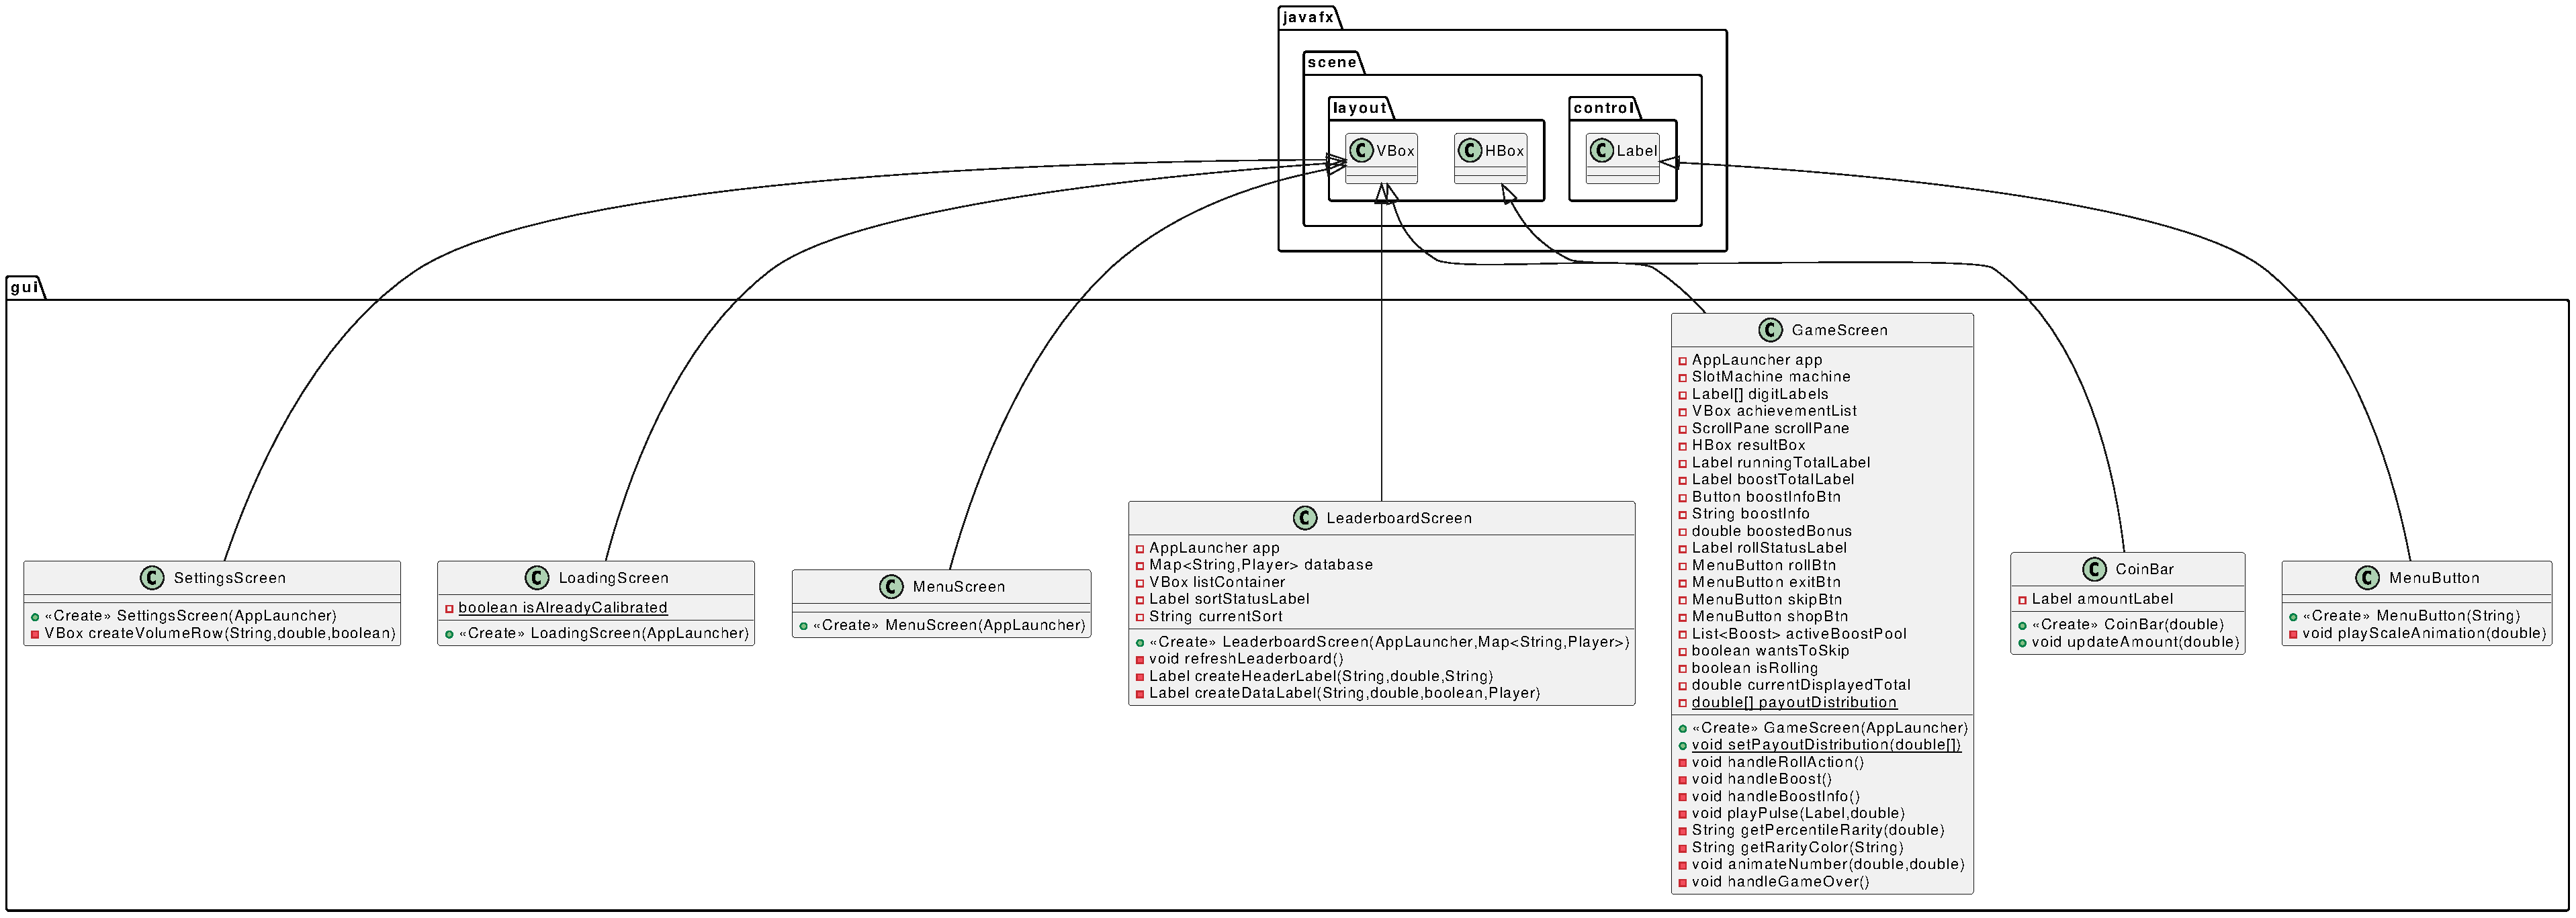
\includegraphics[scale=0.29]{UML/gui2.pdf}}

    \caption{UML of package \texttt{gui}}
\end{figure}

\begin{figure}
    \centering
    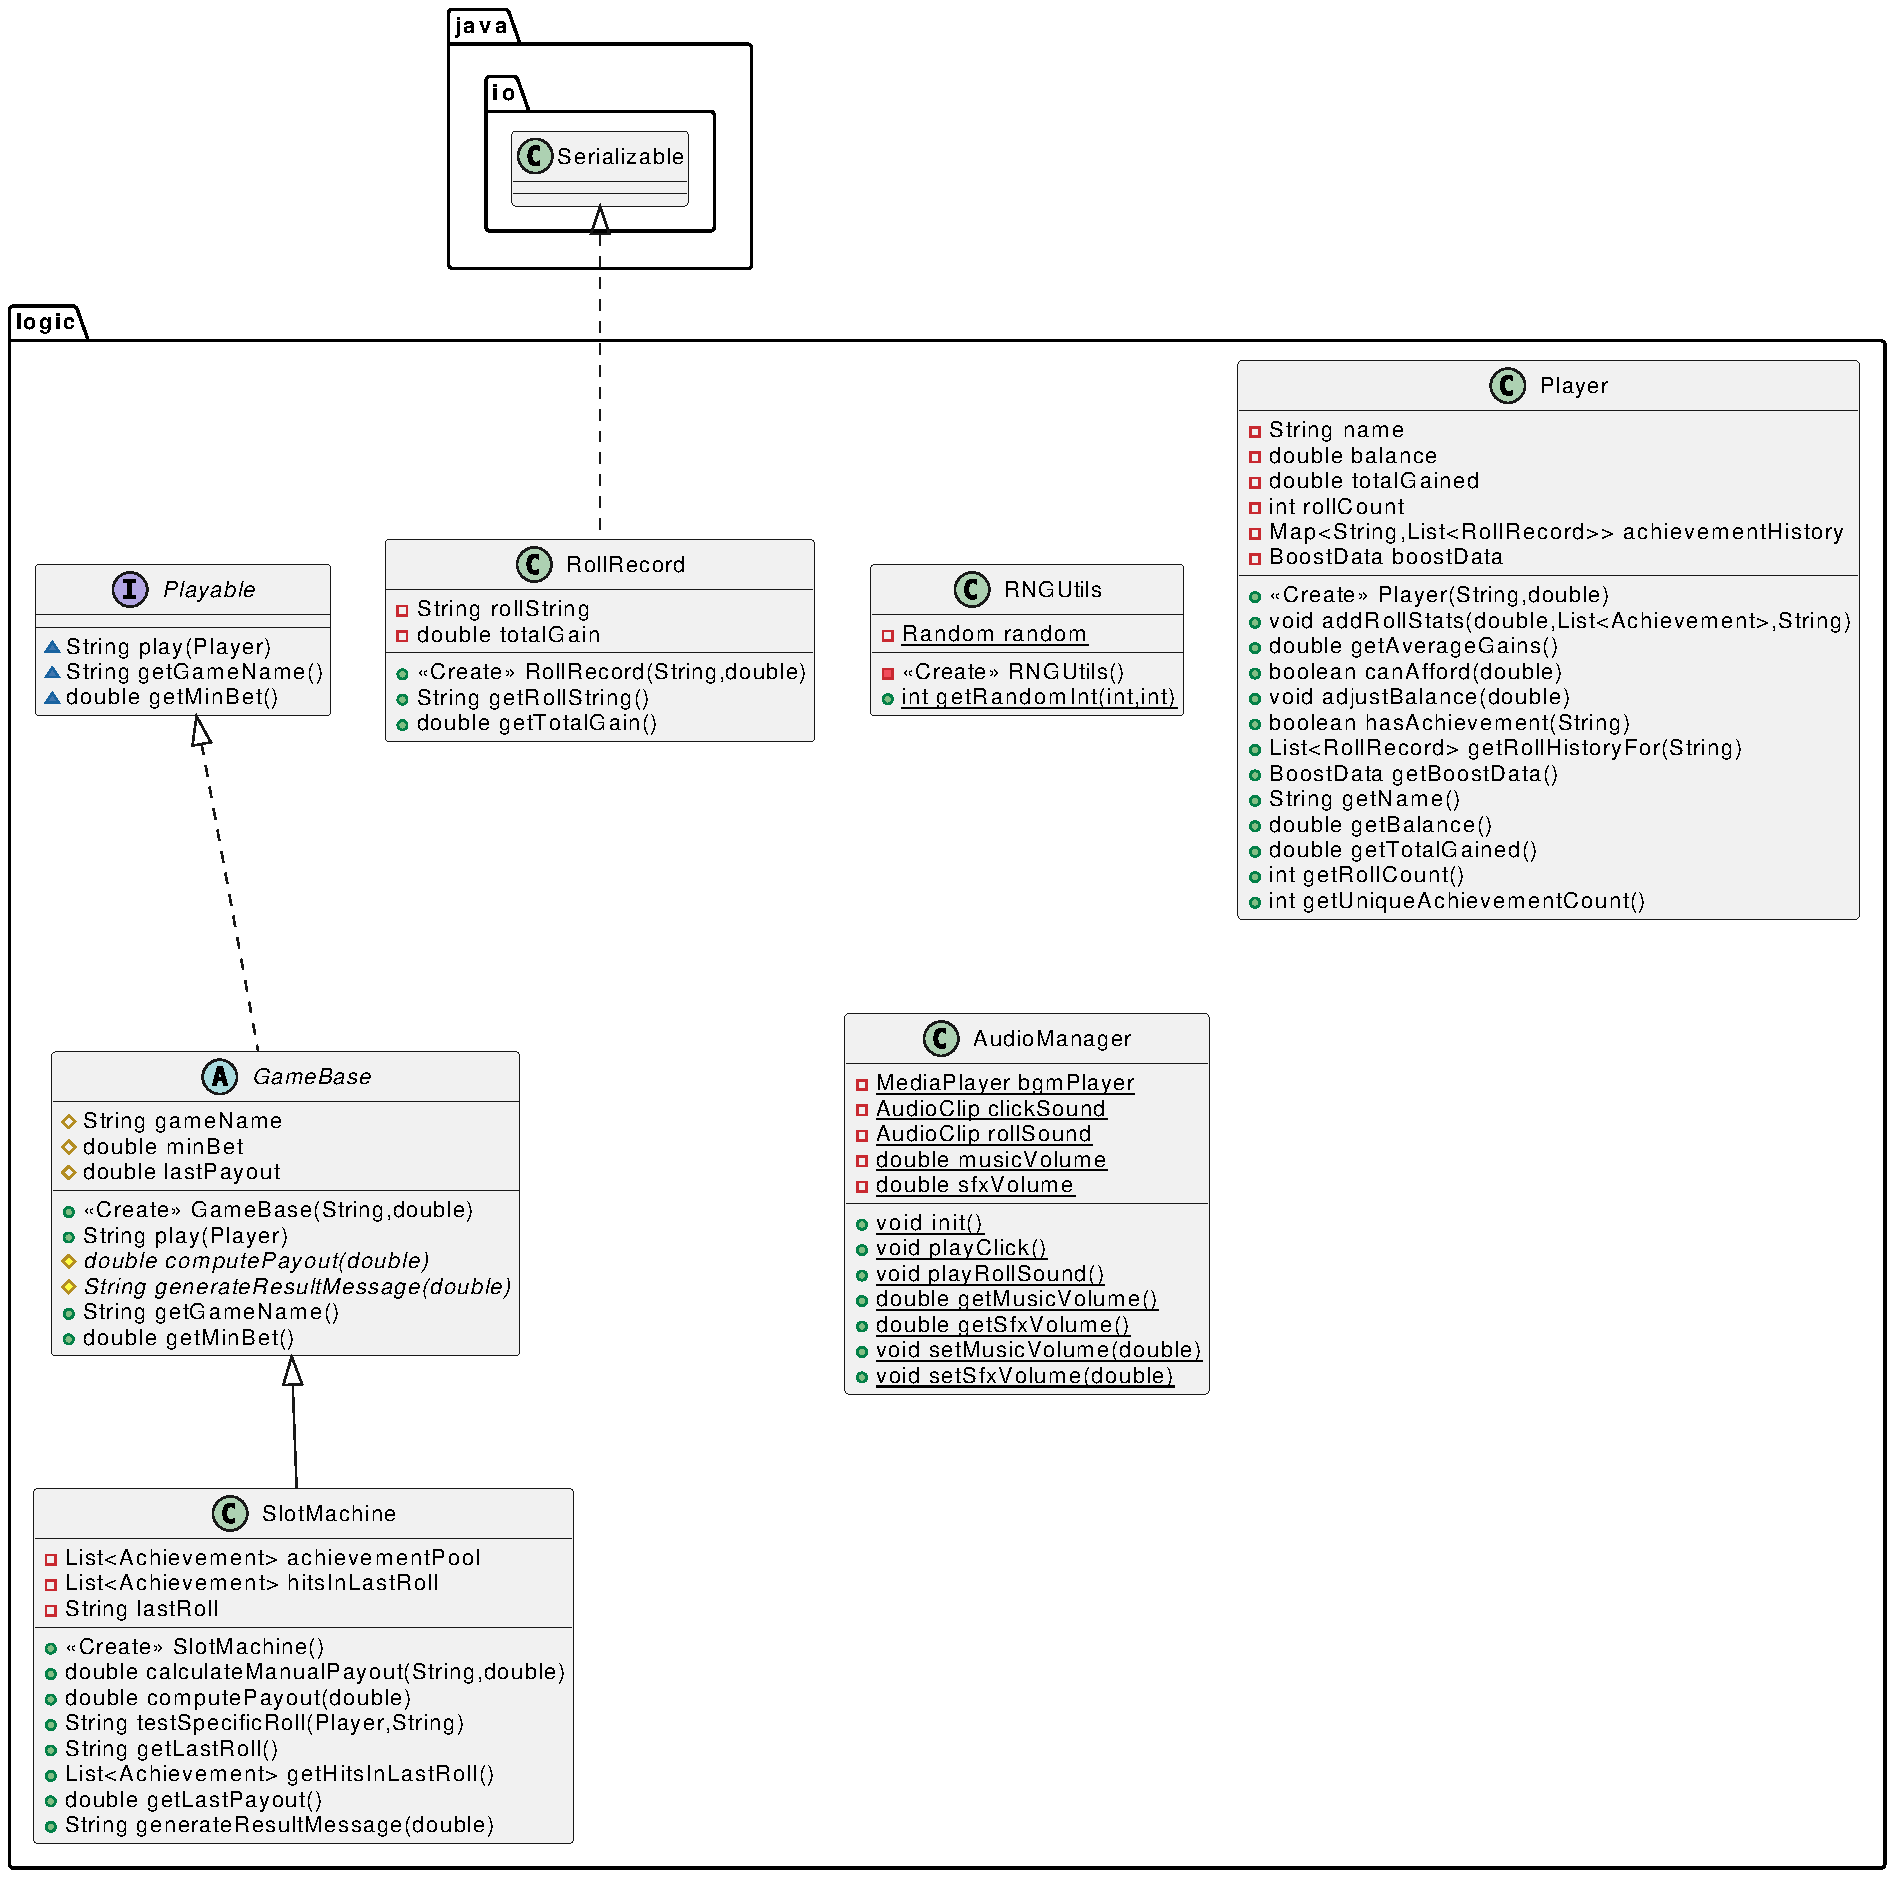
\includegraphics[scale=0.4]{UML/logicBase.pdf}
    \caption{UML of package \texttt{logic}}
\end{figure}

\begin{figure}
    \centering
    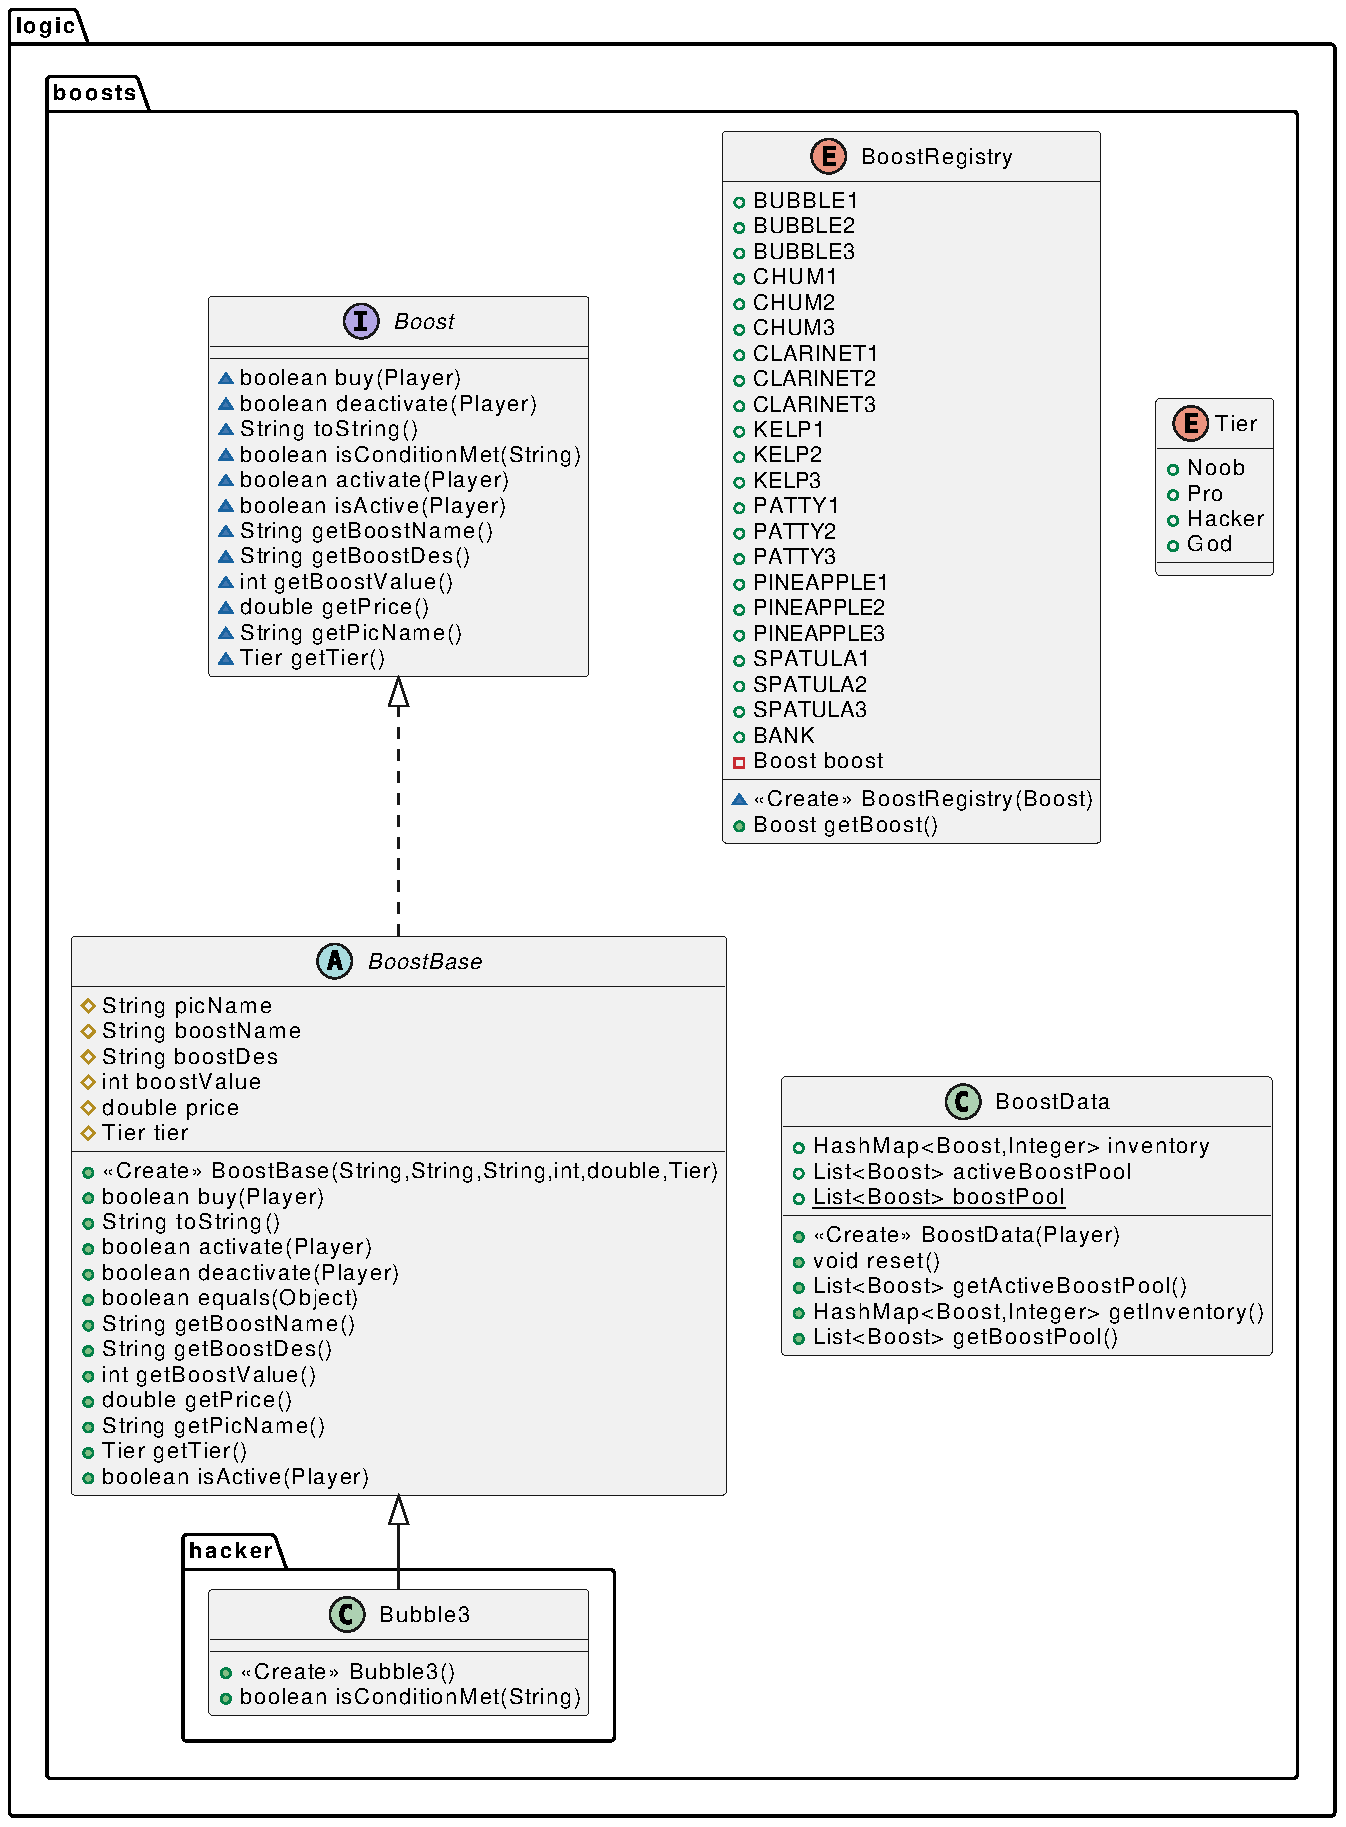
\includegraphics[scale=0.4]{UML/boost.pdf}
    \caption{UML of package \texttt{logic.boosts}*}
\end{figure}

\begin{figure}
    \centering
    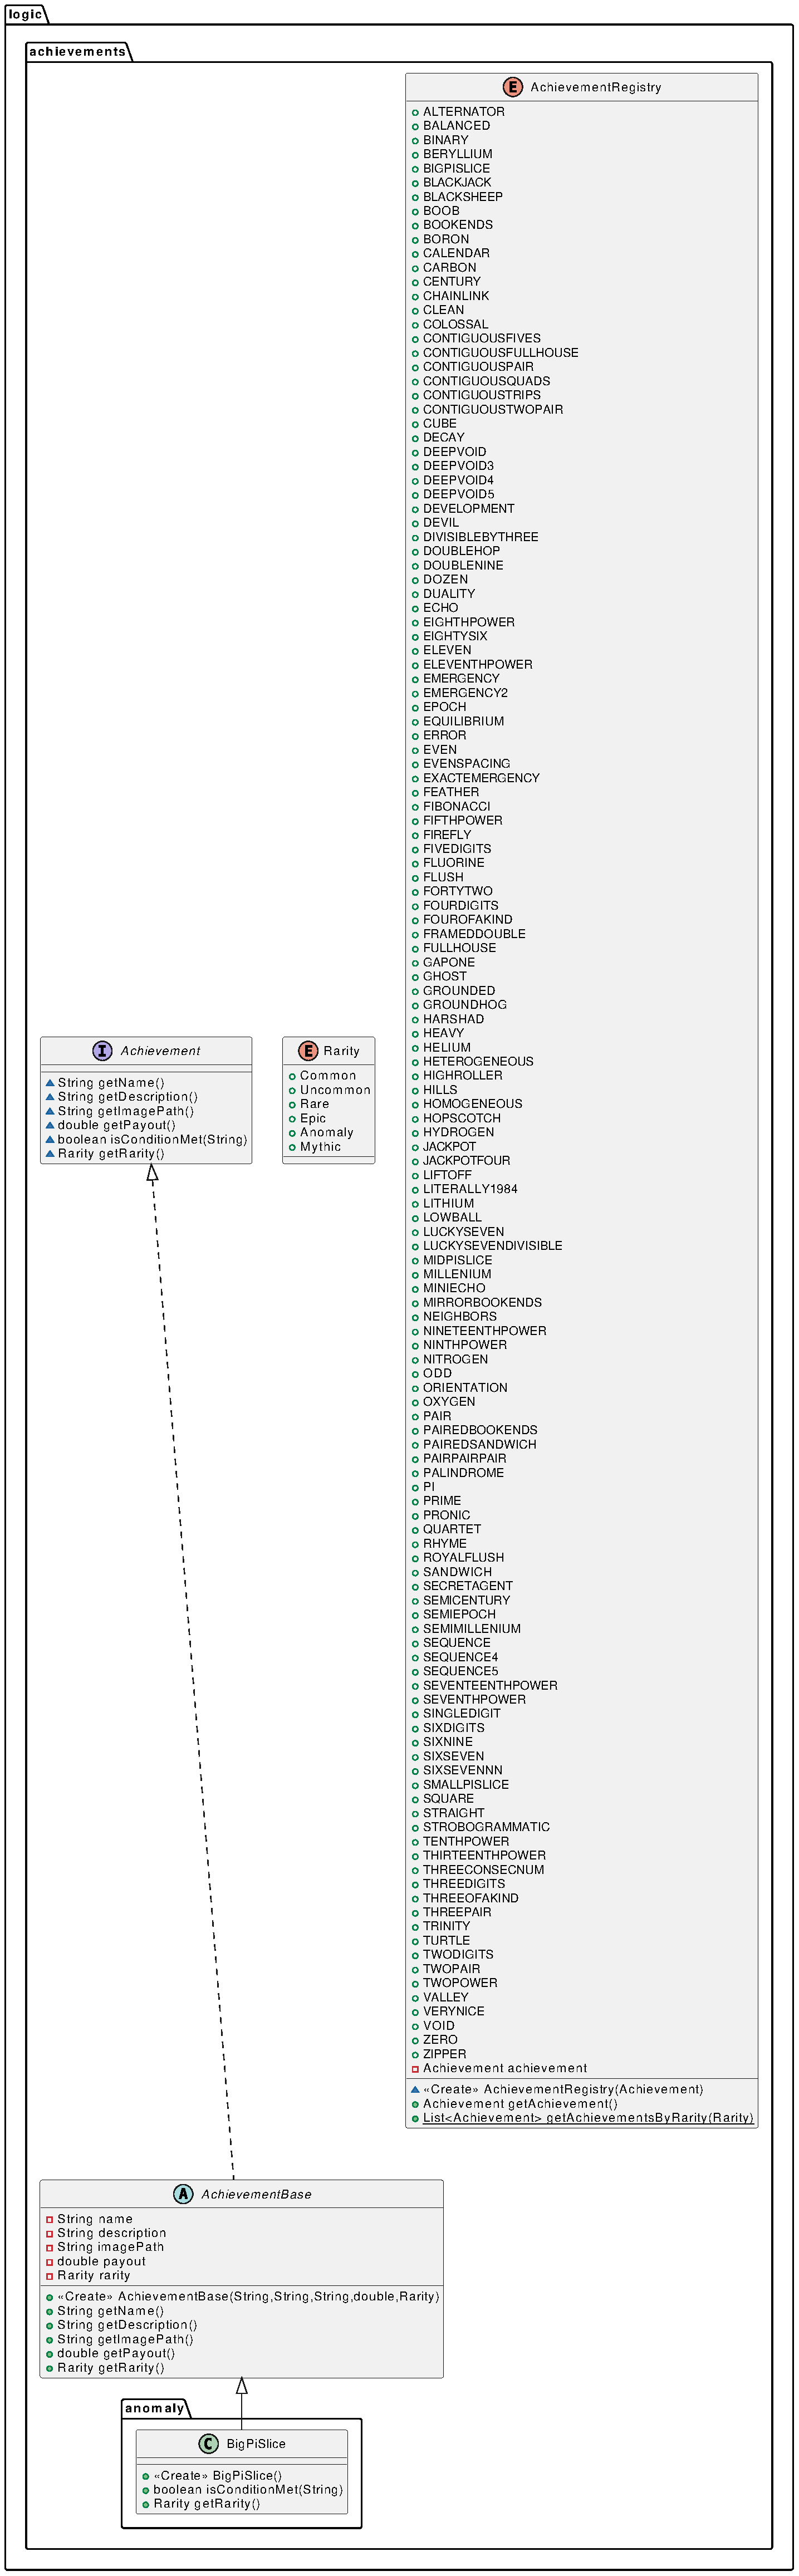
\includegraphics[scale=0.32]{UML/achievement.pdf}
    \caption{UML of package \texttt{logic.achievements}*}
\end{figure}

\restoregeometry
\pagestyle{fancy}

\noindent * These are classes that aren't included to the UML diagram because there are way too many to show.
However, there is already an example class included to represent \emph{boost} (\texttt{Bubble3}) and \emph{achievement} (\texttt{BigPiSlice}) which the rest are all equivalent to.
\bigskip

\noindent{\texttt{logic.achievements.anomaly}}
\begin{multicols}4
    \begin{enumerate}
        \item \texttt{BigPiSlice}
        \item \texttt{Binary}
        \item \texttt{Epoch}
        \item \texttt{Fibonacci}
        \item \texttt{FifthPower}
        \item \texttt{Homogeneous}
        \item \texttt{Millenium}
        \item \texttt{Pi}
        \item \texttt{RoyalFlush}
        \item \texttt{SemiEpoch}
        \item \texttt{TwoDigits}
        \item \texttt{TwoPower}
    \end{enumerate}
\end{multicols}

\noindent{\texttt{logic.achievements.common}}
\begin{multicols}4
    \begin{enumerate}
        \item \texttt{Beryllium}
        \item \texttt{Boron}
        \item \texttt{Carbon}
        \item \texttt{ContiguousPair}
        \item \texttt{Even}
        \item \texttt{Fluorine}
        \item \texttt{GapOne}
        \item \texttt{Ghost}
        \item \texttt{Grounded}
        \item \texttt{Helium}
        \item \texttt{Heterogeneous}
        \item \texttt{Hills}
        \item \texttt{Hopscotch}
        \item \texttt{Hydrogen}
        \item \texttt{LiftOff}
        \item \texttt{Lithium}
        \item \texttt{LuckySeven}
        \item {\footnotesize\texttt{LuckySevenDivisible}}\vphantom{a}
        \item \texttt{Neighbors}
        \item \texttt{Nitrogen}
        \item \texttt{Odd}
        \item \texttt{Oxygen}
        \item \texttt{Pair}
        \item \texttt{Quartet}
        \item \texttt{SixDigits}
        \item \texttt{ThreeKind}
        \item \texttt{TwoPair}
        \item \texttt{Void}
    \end{enumerate}
\end{multicols}

\noindent{\texttt{logic.achievements.epic}}
\begin{multicols}4
    \begin{enumerate}
        \item \texttt{Boob}
        \item \texttt{Colossal}
        \item \texttt{ContiguousFives}
        \item \texttt{Cube}
        \item \texttt{Decay}
        \item \texttt{DeepVoid4}
        \item \texttt{Development}
        \item \texttt{Echo}
        \item \texttt{Emergency2}
        \item \texttt{JackpotFour}
        \item \texttt{Literally1984}
        \item \texttt{MidPiSlice}
        \item \texttt{PairPairPair}
        \item \texttt{Palindrome}
        \item \texttt{Pronic}
        \item \texttt{SemiMillenium}
        \item \texttt{Sequence5}
        \item \texttt{SixSevennn}
        \item \texttt{Straight}
        \item \texttt{Strobogrammatic}
        \item \texttt{ThreeConsecNum}
        \item \texttt{ThreeDigits}
        \item \texttt{VeryNice}
        \item \texttt{Zipper}
    \end{enumerate}
\end{multicols}

\noindent{\texttt{logic.achievements.mythic}}
\begin{multicols}4
    \begin{enumerate}
        \item \texttt{DeepVoid5}
        \item \texttt{EighthPower}
        \item \texttt{EleventhPower}
        \item \texttt{ExactEmergency}
        \item \texttt{Groundhog}
        \item \texttt{NineteenthPower}
        \item \texttt{NinthPower}
        \item \texttt{SeventeenthPower}
        \item \texttt{SeventhPower}
        \item \texttt{SingleDigit}
        \item \texttt{TenthPower}
        \item \texttt{ThirteenthPower}
        \item \texttt{Zero}
    \end{enumerate}
\end{multicols}

\clearpage

\noindent{\texttt{logic.achievements.rare}}
\begin{multicols}4
    \begin{enumerate}
        \item \texttt{BlackSheep}
        \item \texttt{Bookends}
        \item \texttt{Calendar}
        \item \texttt{Century}
        \item {\footnotesize\texttt{ContiguousFullHouse}}\vphantom{a}
        \item \texttt{ContiguousQuads}
        \item \texttt{DeepVoid3}
        \item \texttt{Devil}
        \item \texttt{DivisibleByThree}
        \item \texttt{DoubleNine}
        \item \texttt{Duality}
        \item \texttt{Emergency}
        \item \texttt{Error}
        \item \texttt{EvenSpacing}
        \item \texttt{Firefly}
        \item \texttt{FourDigits}
        \item \texttt{FramedDouble}
        \item \texttt{Heavy}
        \item \texttt{Jackpot}
        \item \texttt{MirrorBookends}
        \item \texttt{Orientation}
        \item \texttt{PairedBookends}
        \item \texttt{PairedSandwich}
        \item \texttt{SecretAgent}
        \item \texttt{SemiCentury}
        \item \texttt{Sequence4}
        \item \texttt{SmallPiSlice}
        \item \texttt{Square}
        \item \texttt{ThreePair}
        \item \texttt{Turtle}
    \end{enumerate}
\end{multicols}

\noindent{\texttt{logic.achievements.uncommon}}
\begin{multicols}4
    \begin{enumerate}
        \item \texttt{Alternator}
        \item \texttt{Balanced}
        \item \texttt{Blackjack}
        \item \texttt{ChainLink}
        \item \texttt{Clean}
        \item \texttt{ContiguousTrips}
        \item {\footnotesize\texttt{ContiguousTwoPair}}\vphantom{a}
        \item \texttt{DeepVoid}
        \item \texttt{DoubleHop}
        \item \texttt{Dozen}
        \item \texttt{EightySix}
        \item \texttt{Eleven}
        \item \texttt{Equilibrium}
        \item \texttt{Feather}
        \item \texttt{FiveDigits}
        \item \texttt{Flush}
        \item \texttt{FortyTwo}
        \item \texttt{FourKind}
        \item \texttt{FullHouse}
        \item \texttt{Harshad}
        \item \texttt{HighRoller}
        \item \texttt{LowBall}
        \item \texttt{MiniEcho}
        \item \texttt{Nice}
        \item \texttt{Peak}
        \item \texttt{Prime}
        \item \texttt{Rhyme}
        \item \texttt{Sandwich}
        \item \texttt{Sequence}
        \item \texttt{SixSeven}
        \item \texttt{Trinity}
        \item \texttt{Valley}
    \end{enumerate}
\end{multicols}

\noindent{\texttt{logic.boosts.hacker}}
\begin{multicols}4
    \begin{enumerate}
        \item \texttt{Bubble3}
        \item \texttt{Chum3}
        \item \texttt{Clarinet3}
        \item \texttt{Kelp3}
        \item \texttt{Patty3}
        \item \texttt{Pineapple3}
        \item \texttt{Spatula3}
    \end{enumerate}
\end{multicols}

\noindent{\texttt{logic.boosts.noob}}
\begin{multicols}4
    \begin{enumerate}
        \item \texttt{Bubble1}
        \item \texttt{Chum1}
        \item \texttt{Clarinet1}
        \item \texttt{Kelp1}
        \item \texttt{Patty1}
        \item \texttt{Pineapple1}
        \item \texttt{Spatula1}
    \end{enumerate}
\end{multicols}

\noindent{\texttt{logic.boosts.pro}}
\begin{multicols}4
    \begin{enumerate}
        \item \texttt{Bubble2}
        \item \texttt{Chum2}
        \item \texttt{Clarinet2}
        \item \texttt{Kelp2}
        \item \texttt{Patty2}
        \item \texttt{Pineapple2}
        \item \texttt{Spatula2}
    \end{enumerate}
\end{multicols}
